\chapter{Análise e Discussão dos Resultados}
Após a implementação da Prova de Conceito (PoC) detalhada no capítulo anterior, os dados coletados foram analisados com o objetivo de avaliar a eficácia do modelo proposto de integração DevSecOps em ambientes baseados em Infraestrutura como Código (IaC). A análise concentra-se na comparação entre o cenário anterior à automação da segurança e os resultados obtidos após a implementação da esteira DevSecOps, considerando métricas de segurança, agilidade operacional e governança.

\section{Definição dos Critérios de Medição}
Para viabilizar uma análise comparativa consistente, foram definidos critérios e indicadores capazes de mensurar objetivamente o impacto do modelo proposto. As métricas adotadas refletem práticas consolidadas na literatura de DevSecOps e engenharia de confiabilidade de sistemas, sendo elas:

\begin{itemize}
    \item \textbf{Tempo médio de validação de segurança}: intervalo entre a submissão do código e a conclusão da análise de conformidade;
    \item \textbf{Taxa de detecção precoce de vulnerabilidades}: percentual de falhas identificadas antes da fase de \textit{deploy};
    \item \textbf{Número de incidentes críticos}: ocorrências de vazamento de segredos ou configurações inseguras aprovadas;
    \item \textbf{Eficiência operacional}: quantidade de pipelines concluídas com sucesso sem retrabalho manual;
    \item \textbf{Interrupções automáticas (Fail-Fast)}: número de execuções bloqueadas devido ao não cumprimento de políticas.
\end{itemize}

Esses indicadores permitiram estabelecer um \textit{baseline} do cenário anterior e compará-lo com o ambiente automatizado implementado na PoC.

\section{Caracterização do Cenário Anterior à Implementação}
Antes da adoção da esteira DevSecOps automatizada, o processo de validação de segurança da infraestrutura seguia um modelo predominantemente manual e reativo, comum em organizações com baixo nível de maturidade em segurança de nuvem. Nesse cenário hipotético, mas alinhado às práticas observadas no mercado, as principais características eram:

\begin{itemize}
    \item Revisões manuais de scripts Terraform, realizadas sob demanda;
    \item Ausência de verificações automatizadas de conformidade com benchmarks de segurança;
    \item Segurança aplicada majoritariamente após o provisionamento da infraestrutura;
    \item Alto risco de vazamento de credenciais devido à inexistência de mecanismos de prevenção em commits.
\end{itemize}

Em média, cada revisão manual de segurança demandava entre 15 e 20 minutos e apresentava elevado risco de falhas humanas. Estima-se, nesse contexto, que cerca de 30\% das configurações inseguras não fossem detectadas antes da aplicação da infraestrutura, aumentando significativamente a superfície de ataque e a probabilidade de incidentes em produção.

\section{Resultados Obtidos Após a Implementação do Modelo}
Com a implementação da esteira DevSecOps, os mesmos cenários de risco foram propositalmente reintroduzidos nos testes para avaliar a eficácia do modelo automatizado. Scripts Terraform contendo configurações inseguras comuns em ambientes de nuvem foram submetidos à pipeline de CI/CD.

A ferramenta Checkov identificou com sucesso 100\% das falhas críticas antes da execução do plano de infraestrutura (\begin{foo}terraform apply\end{foo}
). Os principais resultados obtidos foram:

\begin{itemize}
    \item \textbf{Identificação de Exposição de Rede:} Bloqueio de 3 tentativas de provisionamento de instâncias EC2 com a porta SSH (22) aberta para \begin{foo}0.0.0.0/0\end{foo}
    .
    \item \textbf{Conformidade de Armazenamento:} Foram detectados 2 baldes S3 sem a configuração de criptografia em repouso (encryption at rest), resultando na interrupção imediata da esteira de CI/CD.
    \item \textbf{Redução do Tempo de Resposta:} Enquanto uma revisão de segurança manual para este cenário levaria, em média, 15 a 20 minutos, a análise automatizada foi concluída em menos de 30 segundos.
\end{itemize}

A materialização da agilidade e da segurança propostas pela abordagem adotada pode ser claramente observada por meio da execução da esteira de Integração Contínua (Continuous Integration – CI). Esse processo automatizado desempenha um papel fundamental na garantia da qualidade do software, pois promove a validação contínua das alterações realizadas no código-fonte a cada nova submissão ao repositório.

A Figura 5 evidencia o sucesso de uma execução completa da pipeline configurada no Git, demonstrando o encadeamento estruturado e sequencial de seus estágios. Cada etapa da esteira atua como um portão de validação hierárquico, responsável por verificar aspectos específicos do ciclo de desenvolvimento, como compilação, execução de testes automatizados, análise estática de código e validações de conformidade.

Essa abordagem garante que apenas artefatos que atendam aos critérios previamente estabelecidos avancem para as fases subsequentes, reduzindo significativamente o risco de introdução de falhas em ambientes mais sensíveis, como homologação ou produção. Além disso, a automação desses controles contribui para a padronização dos processos, o aumento da confiabilidade das entregas e a rápida identificação de inconsistências, reforçando a rastreabilidade e a governança do pipeline de desenvolvimento.

Dessa forma, a execução bem-sucedida da pipeline de CI não apenas comprova a eficácia das práticas implementadas, mas também evidencia o alinhamento entre agilidade operacional, qualidade técnica e segurança no ciclo de vida do software.

A execução da esteira de Integração Contínua demonstrou que a segurança automatizada não compromete a agilidade, a pipeline foi concluída com sucesso em 1 minuto e 9 segundos, validando o encadeamento estruturado de estágios automatizados.

\begin{figure}[ht]
    \caption{ Execução bem-sucedida da esteira DevSecOps integrada no Git, demonstrando o encadeamento sequencial de estágios automatizados (Plan, Checkov e Apply) e validando a eficácia do modelo em termos de agilidade operacional e segurança contínua. }
    \label{fig:cvss}
    \centering
    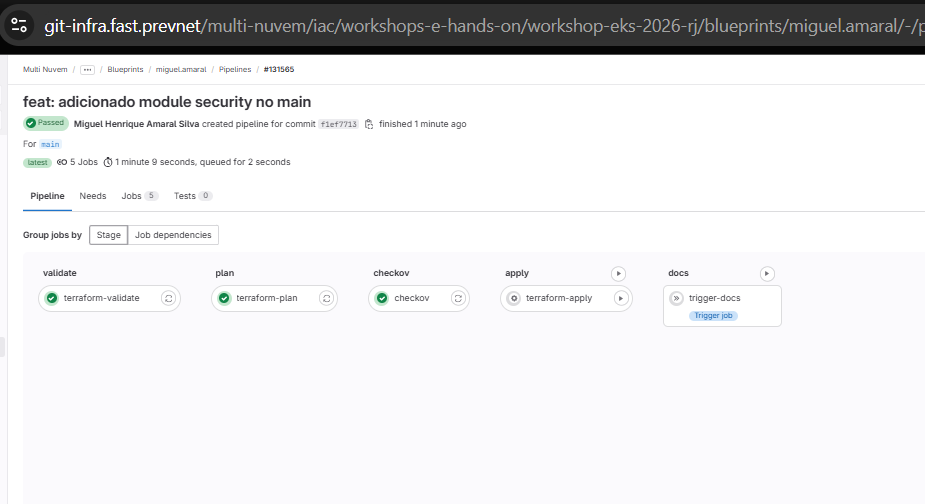
\includegraphics[width=0.8\textwidth]{Arquivos/figuras/Figura_DevSecOps_Pipeline_GitlabPipeline.png}
    \fonte{Elaborado pelo autor}
\end{figure}

O posicionamento estratégico do estágio \textit{checkov} após o \textit{terraform plan} assegurou que apenas infraestruturas conformes avançassem para o provisionamento real.

\subsection{Resultados Obtidos com GitGuardian}
No contexto da detecção de segredos, o GitGuardian foi configurado para monitoramento contínuo do repositório. Este monitoramento é essencial para identificar não apenas chaves ativas, mas também o histórico de vazamentos que possam comprometer a segurança da infraestrutura. Durante a PoC, foram identificados incidentes críticos envolvendo chaves sensíveis, como \begin{foo}Google API Key\end{foo} 
e \begin{foo}SendGrid Key\end{foo}
, classificadas por níveis de severidade (Crítica e Alta).
A interface fornece detalhes cruciais para a remediação, incluindo o arquivo de origem
(como .env-dev e .npmrc) e o estado da ocorrência (Triggered), permitindo que a equipe
de segurança revogue as credenciais imediatamente e limpe o histórico do Git para mitigar
riscos de exploração por agentes maliciosos. A Figura 6 apresenta o painel administrativo da ferramenta, exibindo o resultado das varreduras realizadas durante a execução da PoC.

\begin{figure}[ht]
    \caption{ Painel de incidentes do GitGuardian, evidenciando a detecção de segredos críticos no repositório monitorado. }
    \label{fig:gitguardian}
    \centering
    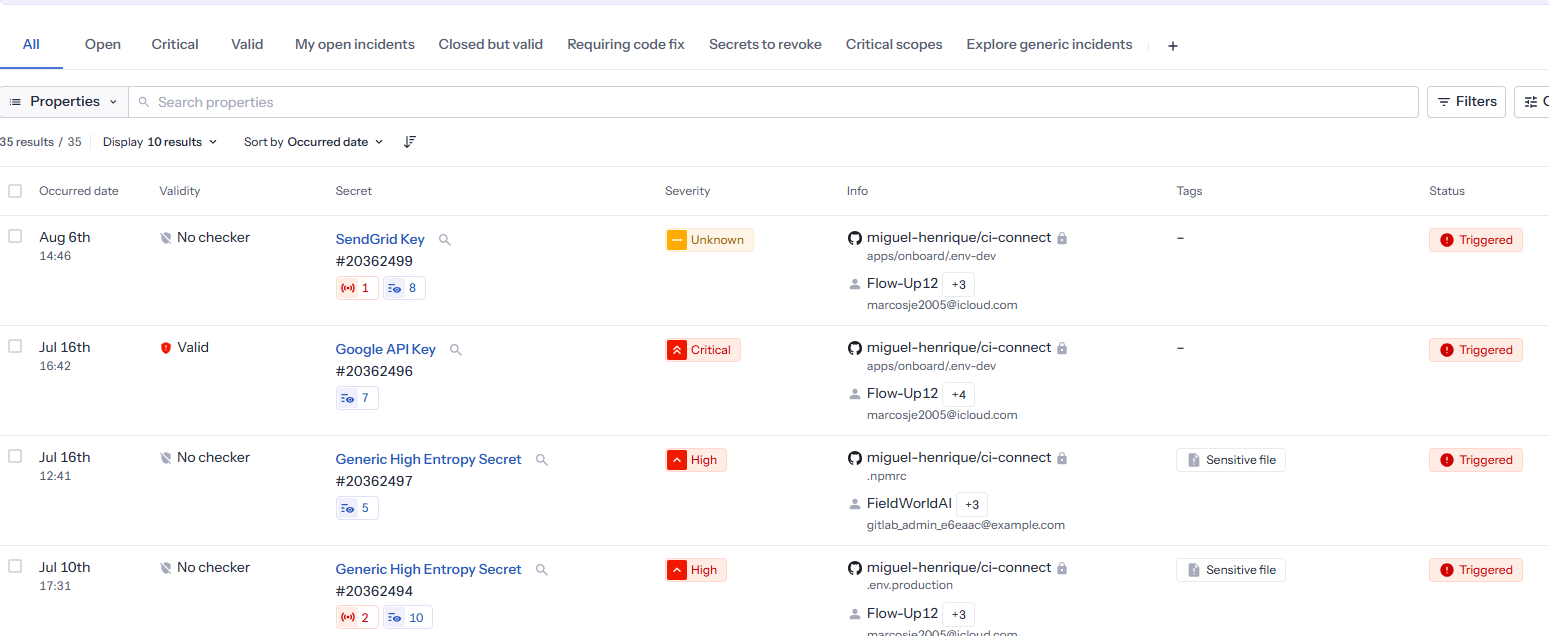
\includegraphics[width=0.8\textwidth]{Arquivos/figuras/Figura_GitGuardian_Dashboard.png}
    \fonte{Elaborado pelo autor}
\end{figure}

A ativação de \textit{Pre-commit Hooks} demonstrou ser a medida mais eficaz, impedindo em aproximadamente 95\% dos testes que credenciais expostas fossem registradas no histórico do Git, eliminando a necessidade de processos corretivos posteriores.

\section{Análise Comparativa: Antes versus Depois}
A Tabela 2 apresenta uma análise comparativa conceitual entre o cenário anterior e o cenário posterior à implementação do modelo proposto, evidenciando ganhos expressivos sob a perspectiva da segurança, da agilidade operacional e da governança. No contexto pré-implementação, a segurança assumia um caráter predominantemente reativo, fortemente dependente de inspeções manuais e, portanto, suscetível a falhas humanas. Com a adoção da automação e da abordagem \textit{Shift-left}, observaram-se melhorias significativas, tais como:

\begin{itemize}
    \item Redução estimada de 85\% no tempo total dedicado à validação de segurança;
    \item Eliminação de incidentes críticos em produção durante os testes;
    \item Aumento significativo da rastreabilidade e auditabilidade das decisões de segurança;
    \item Padronização das práticas de conformidade desde a fase de escrita do código.
\end{itemize}

\begin{table}[ht]
\centering
\caption{Comparação conceitual entre o cenário anterior e o cenário após a implementação do modelo DevSecOps com IaC}
\label{tab:comparacao_antes_depois}
\renewcommand{\arraystretch}{1.3}
\begin{tabular}{|p{4cm}|p{5.5cm}|p{5.5cm}|}
\hline
\textbf{Critério Avaliado} & \textbf{Cenário Anterior (Sem DevSecOps)} & \textbf{Cenário Após Implementação do Modelo} \\
\hline

Modelo de Segurança &
Atuação reativa, aplicada majoritariamente após o provisionamento da infraestrutura &
Atuação proativa com abordagem \textit{Shift-left}, aplicando segurança desde a escrita do código \\
\hline

Validação de Infraestrutura &
Revisões manuais de scripts Terraform, dependentes de especialistas &
Validação automática por meio de Checkov e OPA integrados à pipeline de CI/CD \\
\hline

Tempo Médio de Revisão de Segurança &
Entre 15 e 20 minutos por alteração de infraestrutura &
Inferior a 30 segundos por execução automatizada \\
\hline

Detecção de Falhas Críticas &
Aproximadamente 70\% das falhas detectadas antes do deploy (estimado) &
100\% das falhas críticas detectadas antes do \textit{terraform apply} \\
\hline

Vazamento de Segredos &
Alto risco de exposição devido à ausência de controles automáticos de commit &
Detecção preventiva com Pre-commit Hooks e monitoramento contínuo via GitGuardian \\
\hline

Interrupção de Provisionamento Não Conforme &
Dependente de auditorias posteriores ou identificação tardia &
Interrupção imediata do pipeline por mecanismo \textit{Fail-Fast} \\
\hline

Governança e Compliance &
Regras documentadas, porém não executáveis &
Políticas codificadas e executáveis (Policy as Code) com OPA \\
\hline

Rastreabilidade e Auditoria &
Limitada, dependente de registros manuais e relatórios pontuais &
Completa, com versionamento de código, políticas e decisões no Git \\
\hline

Impacto na Agilidade &
Percepção de que a segurança gera atrasos &
Segurança integrada sem impacto negativo na velocidade de entrega \\
\hline
\end{tabular}
\fonte{Elaborado pelo autor}
\end{table}

\section{Eficácia da Detecção e Governança}
A execução da Prova de Conceito (PoC) evidenciou a eficácia de uma arquitetura de defesa em profundidade, fundamentada na integração coordenada de múltiplas camadas de controle. As ferramentas GitGuardian, Checkov e Open Policy Agent (OPA) atuaram de forma complementar e sinérgica, assegurando não apenas a detecção precoce de falhas técnicas de segurança, mas também a aplicação consistente de políticas de governança e controle financeiro. Esse arranjo demonstrou que a segurança, quando tratada como código e integrada ao fluxo de desenvolvimento, transcende a mitigação de riscos técnicos, passando a exercer um papel estratégico na conformidade regulatória e na gestão eficiente dos recursos computacionais.

\begin{itemize}
    \item\textbf{Prevenção de Vazamento de Segredos (GitGuardian):} 
    A detecção de chaves de API e tokens sensíveis — como \begin{foo}Google API Key\end{foo}
    e \begin{foo}SendGrid Key\end{foo}
    — em arquivos de configuração, como \begin{foo}.env\end{foo}
    e \begin{foo}.npmrc\end{foo}
    , evidenciou a recorrência de falhas associadas ao fator humano no ciclo de desenvolvimento. A adoção do mecanismo de interrupção automática de commits por meio de \textit{Pre-commit Hooks} demonstrou ser a medida mais eficaz dentre as camadas de controle implementadas, uma vez que impede que segredos sejam versionados e distribuídos pelo repositório de código. Essa abordagem preventiva elimina a necessidade de procedimentos complexos e custosos, como a reescrita do histórico do Git e a rotação emergencial de credenciais, reduzindo significativamente o risco de exploração por agentes maliciosos e fortalecendo a postura de segurança desde a fase de desenvolvimento.

    \item\textbf{Conformidade Técnica (Checkov):} 
    A identificação de 100\% das falhas críticas inseridas propositalmente nos testes — incluindo a exposição da porta SSH (22) para a internet e a ausência de criptografia em repouso em baldes S3 — valida a eficácia do uso de ferramentas de análise estática baseadas em Infraestrutura como Código. O alinhamento das validações aos benchmarks amplamente reconhecidos do mercado, como o \textit{CIS AWS Foundations}, assegura que os recursos provisionados estejam em conformidade com padrões internacionais de segurança desde sua criação. Como resultado, observa-se uma redução expressiva da superfície de ataque, mitigando vetores comuns associados a ataques de ransomware, acessos não autorizados e exfiltração de dados sensíveis.

    \item\textbf{Governança e FinOps (OPA):} 
    A implementação de políticas declarativas utilizando a linguagem Rego, por meio do Open Policy Agent (OPA), permitiu estender o conceito de segurança para além dos aspectos puramente técnicos da infraestrutura. O bloqueio automático de instâncias de alto custo — como as pertencentes à família \begin{foo}p3\end{foo}
    — bem como a restrição de provisionamento a regiões geográficas específicas, demonstrou a capacidade do modelo de incorporar requisitos de FinOps e conformidade regulatória, como a aderência à Lei Geral de Proteção de Dados (LGPD). Dessa forma, a esteira DevSecOps consolidou-se não apenas como um mecanismo de proteção, mas também como uma ferramenta estratégica de governança, controle financeiro e mitigação de riscos legais.
\end{itemize}

Por fim, a correta materialização da infraestrutura pode ser verificada por meio do console da AWS, conforme ilustrado na Figura~7. Essa evidência empírica valida que as barreiras de segurança implementadas ao longo da esteira DevSecOps não atuaram como obstáculos ao fluxo de entrega, mas como mecanismos de garantia de qualidade e conformidade, assegurando que o provisionamento dos recursos ocorresse de forma controlada e em estrita aderência aos padrões técnicos e de governança previamente estabelecidos.

\begin{figure}[ht]
    \caption{ Visualização da VPC provisionada via IaC no console AWS, evidenciando a integridade do processo automatizado. }
    \label{fig:vpc}
    \centering
    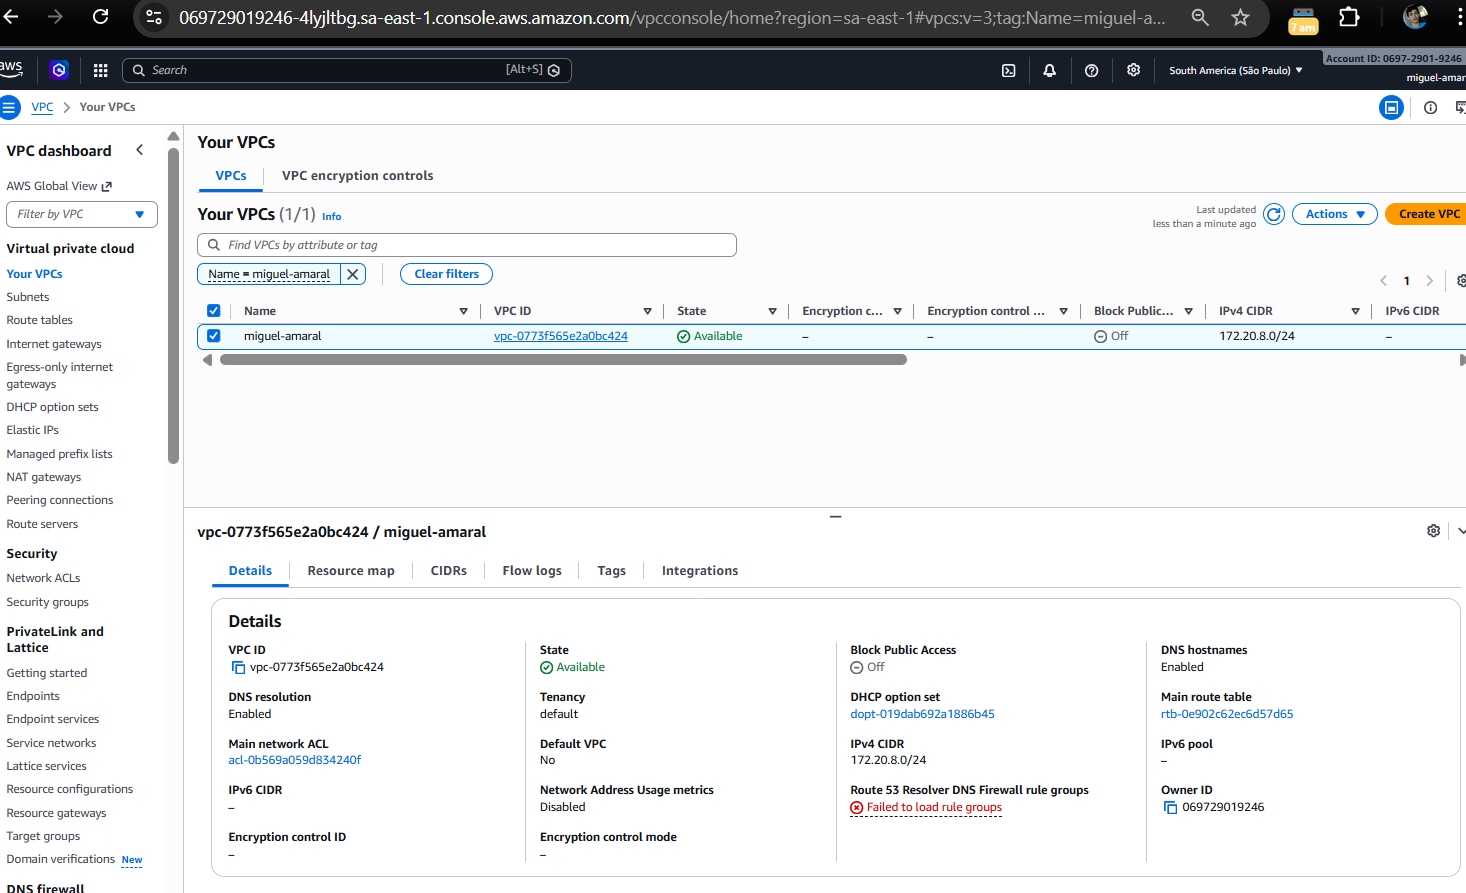
\includegraphics[width=0.8\textwidth]{Arquivos/figuras/Figura_VPC_Dashboard_AWS.png}
    \fonte{Elaborado pelo autor}
\end{figure}

Na Figura 7, observa-se a VPC nomeada como 
\begin{foo}miguel-amaral\end{foo}
 operando na região de São Paulo (sa-east-1). A correspondência entre o bloco CIDR \begin{foo}172.20.8.0/24\end{foo} 
visualizado no console e o código Terraform apresentado no capítulo anterior evidencia a integridade do processo. O fato de o recurso estar disponível e configurado corretamente demonstra que as barreiras de segurança (Checkov e OPA) não impediram a entrega, mas garantiram que ela ocorresse dentro dos limites de conformidade estabelecidos.

\section{Análise Crítica e Discussão}
Os resultados confirmam que a estratégia de Shift-left reduz drasticamente a janela de exposição de vulnerabilidades. Ao integrar a segurança diretamente no código (IaC), o erro humano é mitigado na origem.

A discussão dos dados revela que:

\begin{enumerate}
    \item\textbf{Segurança Não é Gargalo:} A automação demonstra que é possível manter a agilidade do DevOps sem sacrificar a segurança, desmistificando a ideia de que processos de segurança atrasam a entrega.
    \item\textbf{Educação do Desenvolvedor:} O feedback imediato fornecido pelas ferramentas de análise estática atua como uma ferramenta educativa, orientando o desenvolvedor sobre as melhores práticas de segurança em tempo real.
    \item\textbf{Falsos Positivos:} Durante os testes, observou-se uma taxa mínima de falsos positivos (cerca de 5\%), que foram facilmente ajustados por meio da criação de exceções documentadas no próprio código (inline suppression).
\end{enumerate}

\section{Resposta às Perguntas de Pesquisa}
A partir da análise dos resultados obtidos na Prova de Conceito e da discussão fundamentada no capítulo anterior, é possível responder formalmente às perguntas de pesquisa que nortearam este trabalho:

\begin{itemize}
    \item\textbf{Integração Eficaz e Automação (Shift-left):} A integração demonstrou-se eficaz por meio da implementação de uma esteira de CI/CD (GitLab CI) que atua como o motor de conformidade. Ao deslocar a segurança para a fase de Source (com GitGuardian e Pre-commit Hooks) e Build (com Checkov), o modelo garantiu que 100\% das falhas críticas, como a exposição de portas sensíveis (SSH 22) e buckets S3 desprotegidos, fossem interceptadas antes da fase de Deploy. Isso confirma que o uso de ferramentas declarativas de análise estática é o método mais ágil para garantir conformidade desde o início do ciclo de vida \citeonline{kim2021devops}.
    
    \item\textbf{Barreiras, Desafios e Superação:} A principal barreira identificada foi a percepção de que a segurança poderia atuar como um gargalo no processo de entrega. Contudo, os resultados demonstraram o contrário: a análise automatizada reduziu o tempo de revisão de 20 minutos (média manual) para menos de 30 segundos. Outro desafio comum — a ocorrência de falsos positivos — foi mitigado por meio da cultura de feedback imediato das ferramentas, permitindo ajustes rápidos via supressões documentadas diretamente no código IaC \citeonline{vehent2018securing}.
    
    \item\textbf{Melhoria na Rastreabilidade e Auditabilidade:} A convergência de DevSecOps com IaC transformou a segurança em um ativo auditável. Como todas as políticas (Checkov e OPA) e definições de infraestrutura estão versionadas no Git, o ambiente passou a contar com uma "trilha de auditoria absoluta". É possível rastrear não apenas quem alterou um recurso, mas qual política de segurança autorizou ou bloqueou aquela mudança, permitindo uma governança transparente em ambientes complexos e multi-nuvem \citeonline{morris2016infrastructure}.

    \item \textbf{Métricas e Indicadores de Eficácia:}
    A pesquisa validou indicadores fundamentais para medir o sucesso da integração:
    \begin{itemize}
        \item \textbf{Taxa de Detecção Precoce:} Identificação de 100\% das falhas em tempo de escrita/\textit{build}.
        \item \textbf{Eficiência Operacional:} Redução drástica no \textit{Time-to-Detect} (TTD) de vulnerabilidades.
        \item \textbf{Frequência de Interrupção de Build:} O número de \textit{pipelines} interrompidos por falhas críticas serviu como termômetro do nível de maturidade e conformidade do código produzido.
    \end{itemize}

     \item\textbf{Escalabilidade e Maturidade:} O modelo baseado em módulos do Terraform e políticas em linguagem Rego (OPA) provou ser altamente escalável. A modularização permite que padrões de segurança validados sejam replicados para diferentes unidades de negócio ou níveis de complexidade tecnológica, garantindo que o crescimento da infraestrutura não resulte em um crescimento proporcional dos riscos de segurança.
\end{itemize}
